\documentclass{prob}
\usepackage[utf8]{inputenc}
\usepackage{listings}
\usepackage{amsmath}
\usepackage{amsfonts}
\usepackage{amssymb}
\usepackage{amsthm}
\usepackage[spanish,activeacute]{babel}
\usepackage[utf8]{inputenc}
\usepackage{enumerate}
\usepackage{latexsym}
\usepackage{verbatim}
\usepackage{color}
\usepackage{graphicx}
\usepackage{hyperref} % \url
\usepackage{subfig} % \subfloat

% tikz
\usepackage{tikz}
\usetikzlibrary{shapes,arrows,positioning,fit,backgrounds,calc,intersections}
\pgfdeclarelayer{background}
\pgfdeclarelayer{foreground}
\pgfsetlayers{background,main,foreground}
% scale tikz
\usepackage{tikzscale}

\logo{unr2}
\practica{\\ Programación en R}


\newcommand{\real}{\mathbb{R}}
\newcommand{\nat}{\mathbb{N}}


\begin{document}
\maketitle

Esta práctica fue realizada con el objetivo de que los estudiantes tengan un primer acercamiento a la manipulación de datos y a la generación de gráficos adecuados con R, que les será útil para la realización del Trabajo Práctico de Estadística Descriptiva. No es una introducción exhaustiva de la herramienta ni pretende serlo. A lo largo de la práctica se irá guiando al estudiante a la búsqueda y uso de funciones particulares que ayudarán a familiarizarse con el entorno.

\section*{Introducción}
    \begin{problema}
	Una de las primeras tareas a realizar será leer una base de datos proveniente de un archivo. En general, los datos son muchos y no es práctico ingresarlos manualmente. En este caso, se trabajará con el archivo \textit{anorexia.data}\footnote{Disponible para descargar en el sitio de comunidades.}. Dicha base de datos corresponde a una recolección de datos que hizo la \textquotedblleft Asociación de Lucha contra la Bulimia y la Anorexia\textquotedblright durante el mes de octubre del año 2012. La información es acerca de 59 personas con síntomas de anorexia que se habían acercado a la institución en busca de ayuda durante los primeros nueve meses de ese año. Las variables utilizadas son \textquotedblleft Sexo\textquotedblright, \textquotedblleft Cantidad de visitas\textquotedblright , \textquotedblleft Edad \textquotedblright y \textquotedblleft Principal signo visible\textquotedblright (0 - dieta severa, 1 - hiperactividad, 2 - uso de laxantes, 3 - uso de ropa holgada).
	
	\begin{parte}
    	Abra la base de datos con algún editor de texto.\footnote{Esto es recomendable hacerlo únicamente si el archivo tiene un tamaño razonable.} ¿De qué tamaño es la muestra? ¿Cuántas variables se encuentran? ¿Cómo se llaman? ¿De qué tipo son? ¿Cómo está separada una columna de otra?
    \end{parte}
 
	\begin{parte}
    	Lea la base de datos desde R. \\
		
		\noindent\fbox{%
    \parbox{\textwidth}{%
    	\textbf{Ayuda:} puede ser útil buscar la documentación de la función \texttt{read.table()}. ¿Qué argumentos toma? ¿De qué clase es lo que retorna?
    }%
}	

    \end{parte}
        	
    \end{problema}

    \begin{problema}
	Una vez cargada la base de datos, se deben proveer formas de trabajar con las distintas variables. Una manera muy sencilla de acceder a todos los valores de una variable es a través del operador \texttt{\$}:.
	\begin{verbatim}
	    > dataframe_name$variable_name	
	\end{verbatim}
Sin embargo, la notación \$ puede no resultar tan conveniente. La función \texttt{attach()} toma una base de datos (una lista o un  \textit{data frame}) como argumento y hace temporalmente visible sus componentes como variables. La función \texttt{detach()} revierte dicho proceso.
	\begin{verbatim}
	    > attach(dataframe_name)
	    > variable_name	
	\end{verbatim}        	

	\begin{parte}
    	Teniendo en cuenta lo explicado anteriormente, acceda a los contenidos de cada una de las variables por separado. Por ejemplo, para la variable \textquotedblleft Sexo\textquotedblright debería lograr un output similar al siguiente:
    	\begin{verbatim}
        [1] F F F F F F F F F F F F F F F F F F F F F F F F F
       [26] F F F F F F F F F F F F M M M M M M M M M M M M M
       [51] M M M M M M M M M
       Levels: F M
    	\end{verbatim}
    \end{parte}

	\begin{parte}
		Utilizando la función \texttt{class()}, averigue de qué clase es cada variable.   
    \end{parte}

	\begin{parte}
		Cuente la cantidad de mujeres y de hombres que hay en la base de datos.\\
		
	\noindent\fbox{%
    \parbox{\textwidth}{%
		\textbf{Ayuda:} puede ser útil buscar la documentación de la función \texttt{summary()}.
    }%
}	
		
    \end{parte}
    
	\begin{parte}
		Calcule la edad máxima, la mínima y el promedio de todas las edades.\\
			
\noindent\fbox{%
    \parbox{\textwidth}{%
	 \textbf{Ayuda:} puede ser útil buscar la documentación de las funciones \texttt{summary(), sum(), length(), mean()}.
    }%
}			

    \end{parte}    
    \end{problema}
 
\section*{Tablas de frecuencia}    
    \begin{problema}
    En el caso de las variables cuantitativas, antes de presentar distintos gráficos, puede ser útil resumir los datos en tablas de frecuencias como las que se ejemplifican a continuación en la Figura~\ref{fig:tabla2} y en la Figura~\ref{fig:tabla3}.
    
    \begin{figure}[!ht]
    \centering
    
    \fbox{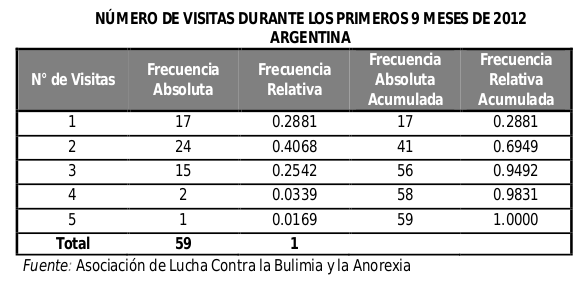
\includegraphics[width=0.55\textwidth]{tabla2.png}}
    \caption{Número de visitas}
    \label{fig:tabla2}
	\end{figure}

    \begin{figure}[!ht]
    \centering
    
    \fbox{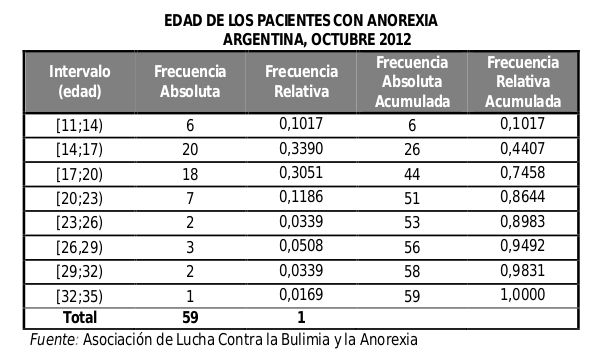
\includegraphics[width=0.55\textwidth]{tabla3.png}}
    \caption{Edad de los pacientes}
    \label{fig:tabla3}
	\end{figure}
	
	\begin{parte}
		Realice la tabla de frecuencias para la variable \textquotedblleft Número de visitas\textquotedblright como se muestra en la Figura~\ref{fig:tabla2} . \\
	
\noindent\fbox{%
    \parbox{\textwidth}{%
		 \textbf{Ayuda:} puede ser útil buscar la documentación de las funciones \texttt{table(), cumsum(), cbind(), rbind(), round(), names()}.
    }%
}	
	\end{parte}
	
	\begin{parte}
		Realice la tabla de frecuencias para la variable \textquotedblleft Edad \textquotedblright como se muestra en la Figura~\ref{fig:tabla3}. ¿Por qué en la fila de esta tabla se encuentran rangos etarios en lugar de valores únicos? \\		
		
		\noindent\fbox{%
    \parbox{\textwidth}{%
		 \textbf{Ayuda:} puede ser útil buscar la documentación de las funciones\texttt{cut(), table(), cumsum(), cbind(), rbind(), round(), names()}.
    }%
}	

	\end{parte}
		
    \end{problema}
        
    \begin{problema}
    Muchas veces es interesante cruzar variables de modo de obtener análisis bivariados. Por ejemplo, en la Figura~\ref{fig:ej3} se presenta una tabla del principal signo visible según el sexo. Observar que en este caso se trata de dos variables cualitativas.\\
\begin{figure}[!ht]
    \centering
    
    \fbox{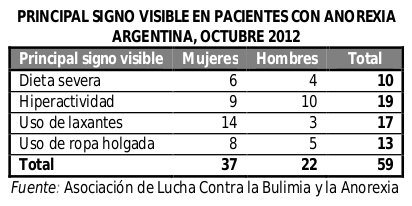
\includegraphics[width=0.45\textwidth]{ej2.png}}
    \caption{Principal signo visible según el sexo}
    \label{fig:ej3}
\end{figure}

	Encuentre la forma de cruzar las variables mencionadas de modo de obtener el contenido de la tabla anterior.\\
	
\noindent\fbox{%
    \parbox{\textwidth}{%
 \textbf{Ayuda:} puede ser útil buscar la documentación de las funciones \texttt{table(), apply(), cbind(), rbind()}.
    }%
}	
	
	\end{problema}
\section*{Gráficos}
Las comodidades para la realización de gráficos son un componente importante y extremadamente versatil del entorno R. Es posible usarlas para producir una amplia variedad de gráficos estadísticos predeterminados así como para construir nuevas clases.\\
A modo general, puede decirse que los comandos de ploteo en R se dividen principalmente en tres grupos:
\begin{itemize}
	\item Alto nivel: crean un nuevo gráfico, posiblemente con títulos, etiquetas, ejes, etc.
	\item Bajo nivel: agregan información a un gráfico ya existente. Por ejemplo: líneas, etiquetas o puntos.
	\item Interactivos: permiten agregar o extraer información interactivamente desde un gráfico ya existente. No serán vistos en esta práctica.
\end{itemize}
Además, R mantiene una lista de parámetros gráficos, los cuales pueden ser manipulados para personalizar los gráficos. A continuación se trabajará con estos conceptos.

	\begin{problema}
	Uno de los tipos de gráficos más utilizados para resumir variables cualitativas es el \textit{diagrama de sectores circulares} o \textit{gráfico de torta}. En la Figura~\ref{fig:plot01} se presenta un ejemplo para la variable \textquotedblleft Principal signo visible\textquotedblright.\\

\begin{figure}[!ht]
    \centering
    
    \fbox{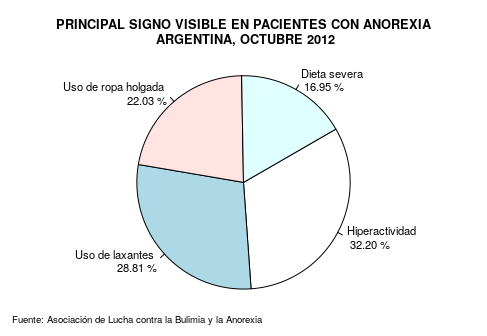
\includegraphics[width=0.6\textwidth]{Rplot01.png}}
    \caption{Principal signo visible}
    \label{fig:plot01}
\end{figure}

	\begin{parte}
		Lea la documentación de la función \texttt{pie()}. ¿Cuál es el significado de los argumentos \texttt{x, labels, clockwise, init.angle} y \texttt{main}?
	\end{parte}

	\begin{parte}
		Realice una primera versión del gráfico de sectores para la variable mencionada, utilizando los argumentos vistos anteriormente. No se preocupe si el gráfico aún no se ve como lo espera.
	\end{parte}	
	
	\begin{parte}	
	En este tipo de gráficos es importante incluir los porcentajes de cada categoría, porque no siempre es claro visualmente si un sector es mayor, menor o igual a otro. Realice una segunda versión del gráfico que tenga en cuenta esto.\\		
		
		\noindent\fbox{%
    \parbox{\textwidth}{%
		 \textbf{Ayuda:} puede ser útil buscar la documentación de la función \texttt{paste()}, y generar un nuevo vector de etiquetas que, además del nombre de cada categoría, contenga el porcentaje que corresponde a cada una.
    }%
}	
	\end{parte}	
	
	\begin{parte}
		Como se mencionó anteriormente, R provee funciones de graficado llamadas \textit{de bajo nivel} que permiten agregar más información a un gráfico ya existente, como líneas, puntos o etiquetas. Una de ellas es \texttt{mtext}, utilizada para escribir texto en los márgenes de un gráfico. Busque la documentación de dicha función. ¿Cuaĺ es el significado de los argumentos \texttt{text, side, line, at, adj, cex} y \texttt{font}? 
	\end{parte}
	
	\begin{parte}
		Realice una tercera versión del gráfico de sectores, utilizando la función estudiada anteriormente.
	\end{parte}
	
	\begin{parte}
		Por último, R provee una función \texttt{par()} utilizada para setear permanentemente o consultar todos los parámetros gráficos. Puede obtener una lista con sus nombres y valores simplemente haciendo:
		\begin{verbatim}
		    > par()
		\end{verbatim}
	Si bien estos parámetros son muchos y no es necesario conocerlos todos, puede ser útil buscar entre ellos cuando se quiera modificar un aspecto particular de los gráficos. Por ejemplo, es posible que le sea conveniente cambiar los valores del parámetro \texttt{mar}, para definir márgenes adecuados en sus gráficos. \\
	
	\textbf{Aclaración:} algunos parámetros específicos de \texttt{par()} pueden pasarse directamente como parámetros en la llamada a la función de alto nivel que grafica. Por ejemplo, es válido hacer lo siguiente:
	\begin{verbatim}
	    > pie(table(Sexo), cex = 0.7,...)
	\end{verbatim}
\medskip	
	Busque la documentación de la función \texttt{par()}. ¿Cuántos parámetros gráficos se pueden setear o consultar a través de ella? ¿Para qué sirve el parámetro \texttt{cex}?
	\end{parte}
		
	\begin{parte}	
	Realice una última versión del gráfico de sectores que se vea similar al que se muestra en la Figura~\ref{fig:plot01}.
	\end{parte}

	\end{problema}
	
	\begin{problema}
	Otro de los tipos de gráficos más utilizados para variables cualitativas es el \textit{gráfico de barras}. En la Figura~\ref{fig:plot02} se presenta un ejemplo, nuevamente para la variable \textquotedblleft Principal signo visible\textquotedblright.\\
	
\begin{figure}[!ht]
    \centering
    
    \fbox{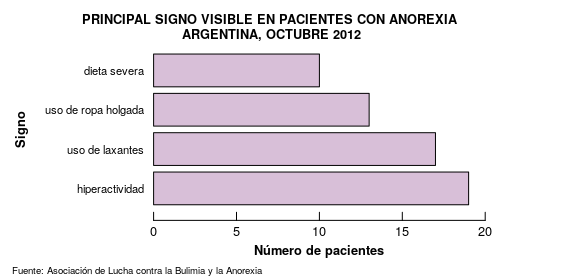
\includegraphics[width=0.6\textwidth]{Rplot02.png}}
    \caption{Principal signo visible}
    \label{fig:plot02}
\end{figure}	
	
	\begin{parte}
		Lea la documentación de la función \texttt{barplot()}. ¿Cuál es el significado de los argumentos \texttt{height, horiz, xlab, ylab, xlim, cex.axis} y \texttt{cex.names}?
	\end{parte}	
	
	\begin{parte}
	Realice una primera versión del gráfico de barras para la variable mencionada, utilizando todo lo visto anteriormente. No se preocupe si el gráfico aún no se ve como lo espera.	
	\end{parte}
	
	\begin{parte}
	Para lograr una mejor percepción visual, las categorías en los gráficos de barras suelen ordenarse de forma creciente o decreciente. Realice una segunda versión del gráfico de barras teniendo en cuenta esto. \\
	
	\noindent\fbox{%
    \parbox{\textwidth}{%
		 \textbf{Ayuda:} puede ser útil buscar la documentación de la función \texttt{order()}.
    }%
}	
	\end{parte}
	
	\begin{parte}
	Setee los parámetros gráficos necesarios y realice una última versión del gráfico que se vea similar al que se presenta en la Figura~\ref{fig:plot02}.
	\end{parte}	
	\end{problema}
	
	\begin{problema}
	Un gráfico de barras compuesto permite comparar resultados para diferentes grupos. Por ejemplo, en la Figura~\ref{fig:plot03} se puede visualizar el principal signo visible según el sexo del paciente.
\begin{figure}[!ht]
    \centering
    
    \fbox{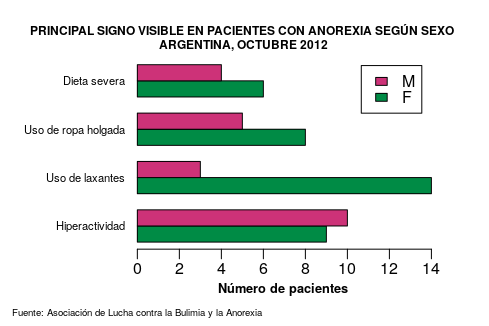
\includegraphics[width=0.6\textwidth]{Rplot03.png}}
    \caption{Principal signo visible}
    \label{fig:plot03}
\end{figure}	

	Realice un gráfico similar, teniendo en cuenta cómo se utiliza la función \texttt{barplot()} cuando el argumento \texttt{height} es una matriz. 

	\end{problema}

	\newpage
	
	\begin{problema}
	Para representar gráficamente datos de variables discretas, especialmente cuando toman pocos valores diferentes, se puede utilizar un \textit{gráfico de bastones}. Por ejemplo, en la Figura~\ref{fig:bast} se muestra un gráfico de bastones correspondiente al número de visitas a la asociación por paciente. 

\begin{figure}[!ht]
    \centering
    
    \fbox{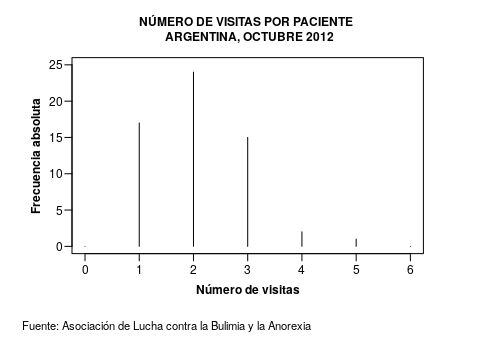
\includegraphics[width=0.6\textwidth]{bast.png}}
    \caption{Número de visitas por paciente}
    \label{fig:bast}
\end{figure}		
	
	\begin{parte}
	Busque la documentación de la función \texttt{plot()}. Observe que la descripción dice \textquotedblleft Función genérica para graficar objetos de R\textquotedblright . La idea de \textit{función genérica} implica, en este caso, que el tipo de gráfico generado por \texttt{plot()} dependerá del tipo o clase de su primer argumento. A continuación, se presentan algunos ejemplos de posibles llamadas:
	\begin{itemize}
	\item \texttt{plot(x, y)}: si \texttt{x} e \texttt{y} son vectores, el resultado será un diagrama de dispersión \footnote{Un diagrama de dispersión es un gráfico que utiliza las coordenadas cartesianas para mostrar los valores de dos variables para un conjunto de datos.}
	\item \texttt{plot(f)}: si \texttt{f} es un factor, entonces generará un gráfico de barras.
	\item \texttt{plot(f,y)}: si \texttt{f} es un factor e \texttt{y}, un vector numérico, la llamada producirá un \textit{boxplot comparativo}\footnote{Vea el ejercicio 10.}.
	\end{itemize}		
	A su vez, \texttt{plot()} cuenta con un parámetro \texttt{type}. Estudie los distintos gráficos que puede realizar a través de dicho argumento.
	\end{parte}
	
	\begin{parte}
	Realice un gráfico de bastones similar al de la Figura~\ref{fig:bast} utlizando la función \texttt{plot()} y lo visto anteriormente. 
	\end{parte}

	\begin{parte}
	Los gráficos de bastones suelen ir acompañados por  \textit{gráficos escalonados} que se utilizan para mostrar la distribución acumulada de una variable discreta. En la Figura~\ref{fig:bast2} se muestra el ejemplo correspondiente al caso trabajado. Confeccione dicho gráfico a través de la función \texttt{plot()}.\\
	
	\noindent\fbox{%
    \parbox{\textwidth}{%
		 \textbf{Ayuda:} puede ser útil buscar la documentación de la función \texttt{abline()} para agregar líneas punteadas de referencia.
    }%
}
	\end{parte}

\begin{figure}[!ht]
    \centering
    
    \fbox{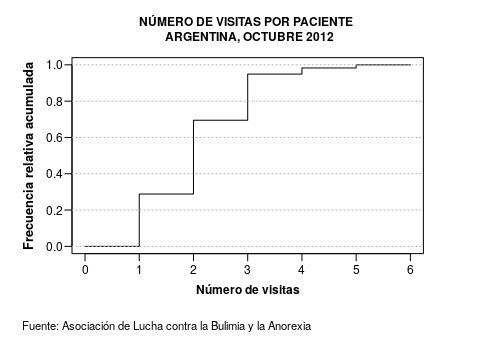
\includegraphics[width=0.6\textwidth]{bast2.png}}
    \caption{Número de visitas por paciente}
    \label{fig:bast2}
\end{figure}	
	
	\end{problema}
	
	\begin{problema}
	En el caso de las variables continuas o discretas que asumen muchos valores distintos, suele utilizarse un \textit{histograma} para representarlas gráficamente. En la Figura~\ref{fig:hist} se puede ver el histograma correspondiente a la edad de los pacientes. \\
	\textbf{Observación:} los intervalos etarios utilizados en el gráfico coinciden con los de la correspondiente tabla de frecuencias.
\begin{figure}[!ht]
    \centering
    
    \fbox{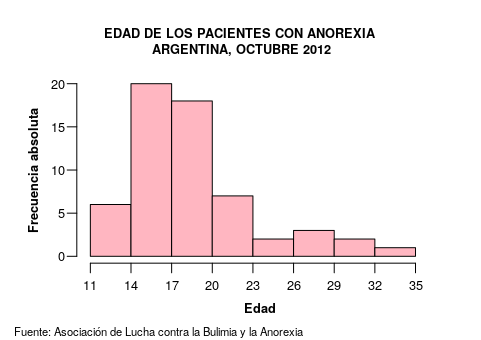
\includegraphics[width=0.6\textwidth]{hist.png}}
    \caption{Edad de los pacientes}
    \label{fig:hist}
\end{figure}		
	
	\begin{parte}
	Busque la documentación de la función \texttt{hist()}. ¿Para qué sirven los argumentos \texttt{breaks} y \texttt{right}? Utilice dicha función para generar el histograma presentado anteriormente.\\
	
	\noindent\fbox{%
    \parbox{\textwidth}{%
		 \textbf{Ayuda:} puede ser útil buscar la documentación de la función \texttt{axis()} para dibujar los ejes independientemente.
    }%
}
	\end{parte}	
	
	\begin{parte}
	Los histogramas suelen ir acompañados de dos gráficos auxiliares: el \textit{polígono de frecuencias} y el \textit{polígono acumulativo}. En la Figura ~\ref{fig:hist23} se muestran dichos gráficos.

\begin{figure}[!ht]
    \centering
    \subfloat[Polígono de frecuencias]
    {
        \fbox{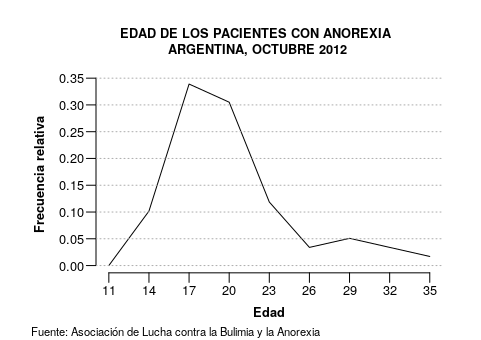
\includegraphics[width=0.45\textwidth]{hist2.png}}
    }
    \subfloat[Polígono acumulativo]
    {
        \fbox{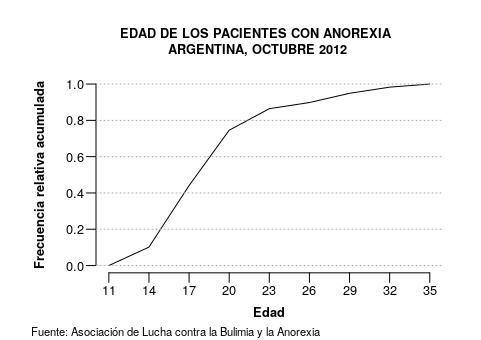
\includegraphics[width=0.45\textwidth]{hist3.png}}
    }
    \caption{Edad de los pacientes}
    \label{fig:hist23}
\end{figure}

	Teniendo en cuenta todas las funciones trabajadas anteriormente, utilice \texttt{plot()} para realizar cada uno de los gráficos. Piense qué valor tomará el argumento \texttt{type} en estos casos.

	\end{parte}
	
	\end{problema}

	\begin{problema}
	El \textit{boxplot} es un gráfico basado en los cinco números resumen de un conjunto de datos: el mínimo, el primer cuartil, la mediana, el tercer cuartil y el máximo. En la Figura ~\ref{fig:boxplot} se muestra un ejemplo de boxplot para la variable \textquotedblleft Edad \textquotedblright .

\begin{figure}[!ht]
    \centering
    
    \fbox{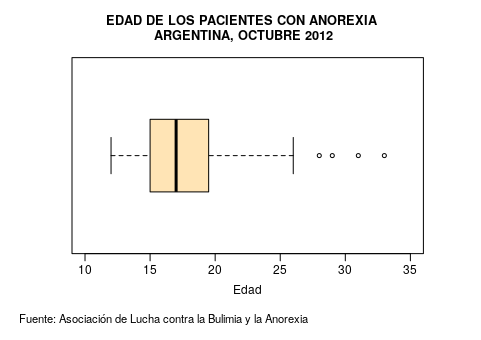
\includegraphics[width=0.55\textwidth]{boxplot.png}}
    \caption{Edad de los pacientes}
    \label{fig:boxplot}
\end{figure}	

	\begin{parte}
	Busque la documentación de la función \texttt{summary()} si no lo hizo antes. Pruébela para cada columna de la base de datos. Compare los resultados para las variables \textquotedblleft Sexo \textquotedblright y \textquotedblleft Número de visitas \textquotedblright . ¿Por qué cree que calcula diferentes medidas en ambos casos? ¿Qué observa al calcular las medidas resúmenes de la variable \textquotedblleft Principal signo visible\textquotedblright ?\\
	
		\noindent\fbox{%
    \parbox{\textwidth}{%
		 El comportamiento anterior se debe a que \texttt{summary()} es una \textit{función genérica}. Como se vio en un ejercicio previo, en R, este tipo de funciones determina la clase de su argumento y usa dicha información para seleccionar el método apropiado. Así, por ejemplo, \texttt{summary()} calcula distintas medidas resúmenes según si el argumento es una variable cualitativa (en general, asociada a un factor) o cuantitativa. Sin embargo, es importante notar que siempre se deben analizar los resultados que devuelve.
    }%
}\\
	
	\end{parte}	
	
	\begin{parte}
	Busque la documentación de la función \texttt{boxplot()} y realice el gráfico de la 	Figura ~\ref{fig:boxplot}.
	\end{parte}
	
	\begin{parte}
	Los boxplots comparativos son muy útiles para la comparación gráfica de distribuciones en grupos
distintos. En la Figura ~\ref{fig:boxplot2} se muestra un ejemplo para la edad según el sexo de los pacientes.

\begin{figure}[!ht]
    \centering
    
    \fbox{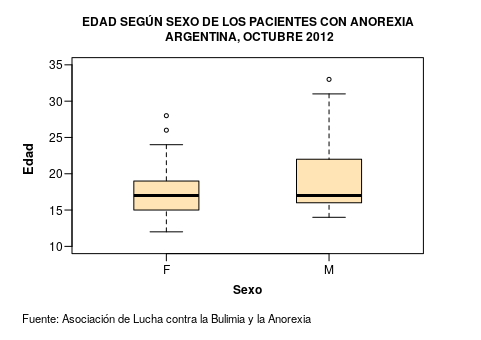
\includegraphics[width=0.55\textwidth]{boxplot2.png}}
    \caption{Edad de los pacientes según el sexo}
    \label{fig:boxplot2}
\end{figure}		 
	\end{parte}

	El gráfico anterior puede ser generado nuevamente con la función \texttt{boxplot()}, utilizando el parámetro \texttt{formula}. Hágalo.\\
	
	\noindent\fbox{%
    \parbox{\textwidth}{%
		 \textbf{Ayuda:} el parámetro \texttt{formula} toma algo de la forma \textit{y $\thicksim$ grp}, donde \texttt{y} es un vector numérico de datos que serán distribuidos en grupos, acordes a la variable \texttt{grp} (usualmente un factor). 

    }%
}
	

	
	\end{problema}
	
\end{document}
